



Die Grundlegende Idee bestand darin eine Frequenzanalyse mit Wavelets zu machen. Diese kann dann gebraucht werden um die Signale nach belieben zu manipulieren und nach wünschen anzupassen. Die Multiskalenanalyse bietet einen schnellen Rechenalgorhytmus jedoch ist er darauf konzipiert keine redundate Daten zu erzeugen. Durch das prinzip der Frequenzhalbierung, die auf jedem sogenannten Level einer Multiskalenanalyse passiert, sieht man nur alle Oktaven eines Signales. So können Frequenzen die nahe bei einander liegen nicht von einander unterschieden werden. Dafür lässt sich das ursprüngliche Signal nach einer msa wieder verlustfrei rekonstruieren.

\subsection{Framing}
Die normale msa besitzt nur Orthonormierte Basen weshalb sie auch keine redundante Daten besitzt. Zur analyse zwecken würde es sich lohnen mehr von diesen Basen zu erzeugen und die enstehung der zusätzlichen Informationen zu verwenden. Wenn wir nun mehr von diesen Basen hinzufügen erschaffen wir ein überbestimmtes System welches ab hier Frame genannt wird. Um ein Frame sinnvoll zu gestalten werden die zusätzlichen Basen auch im Zweierlogharitmus gestaltet. Um nun alle zwölf Halbtöne eines eines Signales detektieren zu können werden mindestens zwölf Basen benötigt. Um ein Sampling herzustellen wird als Grundbasis der Beginn einer Oktave verwendet. Da die Samplingfrequenz mindestens doppelt so schnell sein muss wie die zu Analysierende Frequenz kann als Oktavenbasis ein vielfaches von $220[Hz]$ verwendet werden. Sinnvollerweise auch im zweierlogarhytmus. Das mp3 Format kann eine maximale Tonfrequenz von $16k[Hz]$ wiedergeben. Dem entsprechend ist für Musik eine Maximale Samplingfrequenz von $32k[Hz]$ sinvoll. In der Theorie spielt es jedoch keine Rolle in welchen Frequenzband das Sampling geschieht solange $\frac{f_{Sampling}}{f_{Signal}}\geq2$ gegeben ist. Mit der folgenden Gleichung wurden die verschiednen Samplingfrequenzen bestimmt welche dann verwendet wurden um die Signale neu zu Samplen. 
\begin{equation}
fs_{n}=f*2^{\frac{n}{k}}
\end{equation}
$k$ steht hier für die Anzahl Basen die man in einer Oktave haben möchte. Sinnvollerweise wir $k \geq 12$ gewählt.\\

\subsection{Analyse mit Frames}
In diesem Unterkapitel wird beschrieben welchen ablauf gewählt wurde um eine Analyse eines Testsignales durchzuführen.\\
Zuerst wurde ein Testsignal $x(t)$ erstellt. In der Grafik \ref{fig:frame-testsig} ist $x(t)$ abgebildet. \\
Beschreibung Signal ToDo:\\

In der Grafik \ref{fig:Frame-Analyse} wird eine Frame Analyse und eine cwt Analyse des gleichen Testsignales nebeneinander gestellt. 
\begin{figure}[!ht]
	\centering
	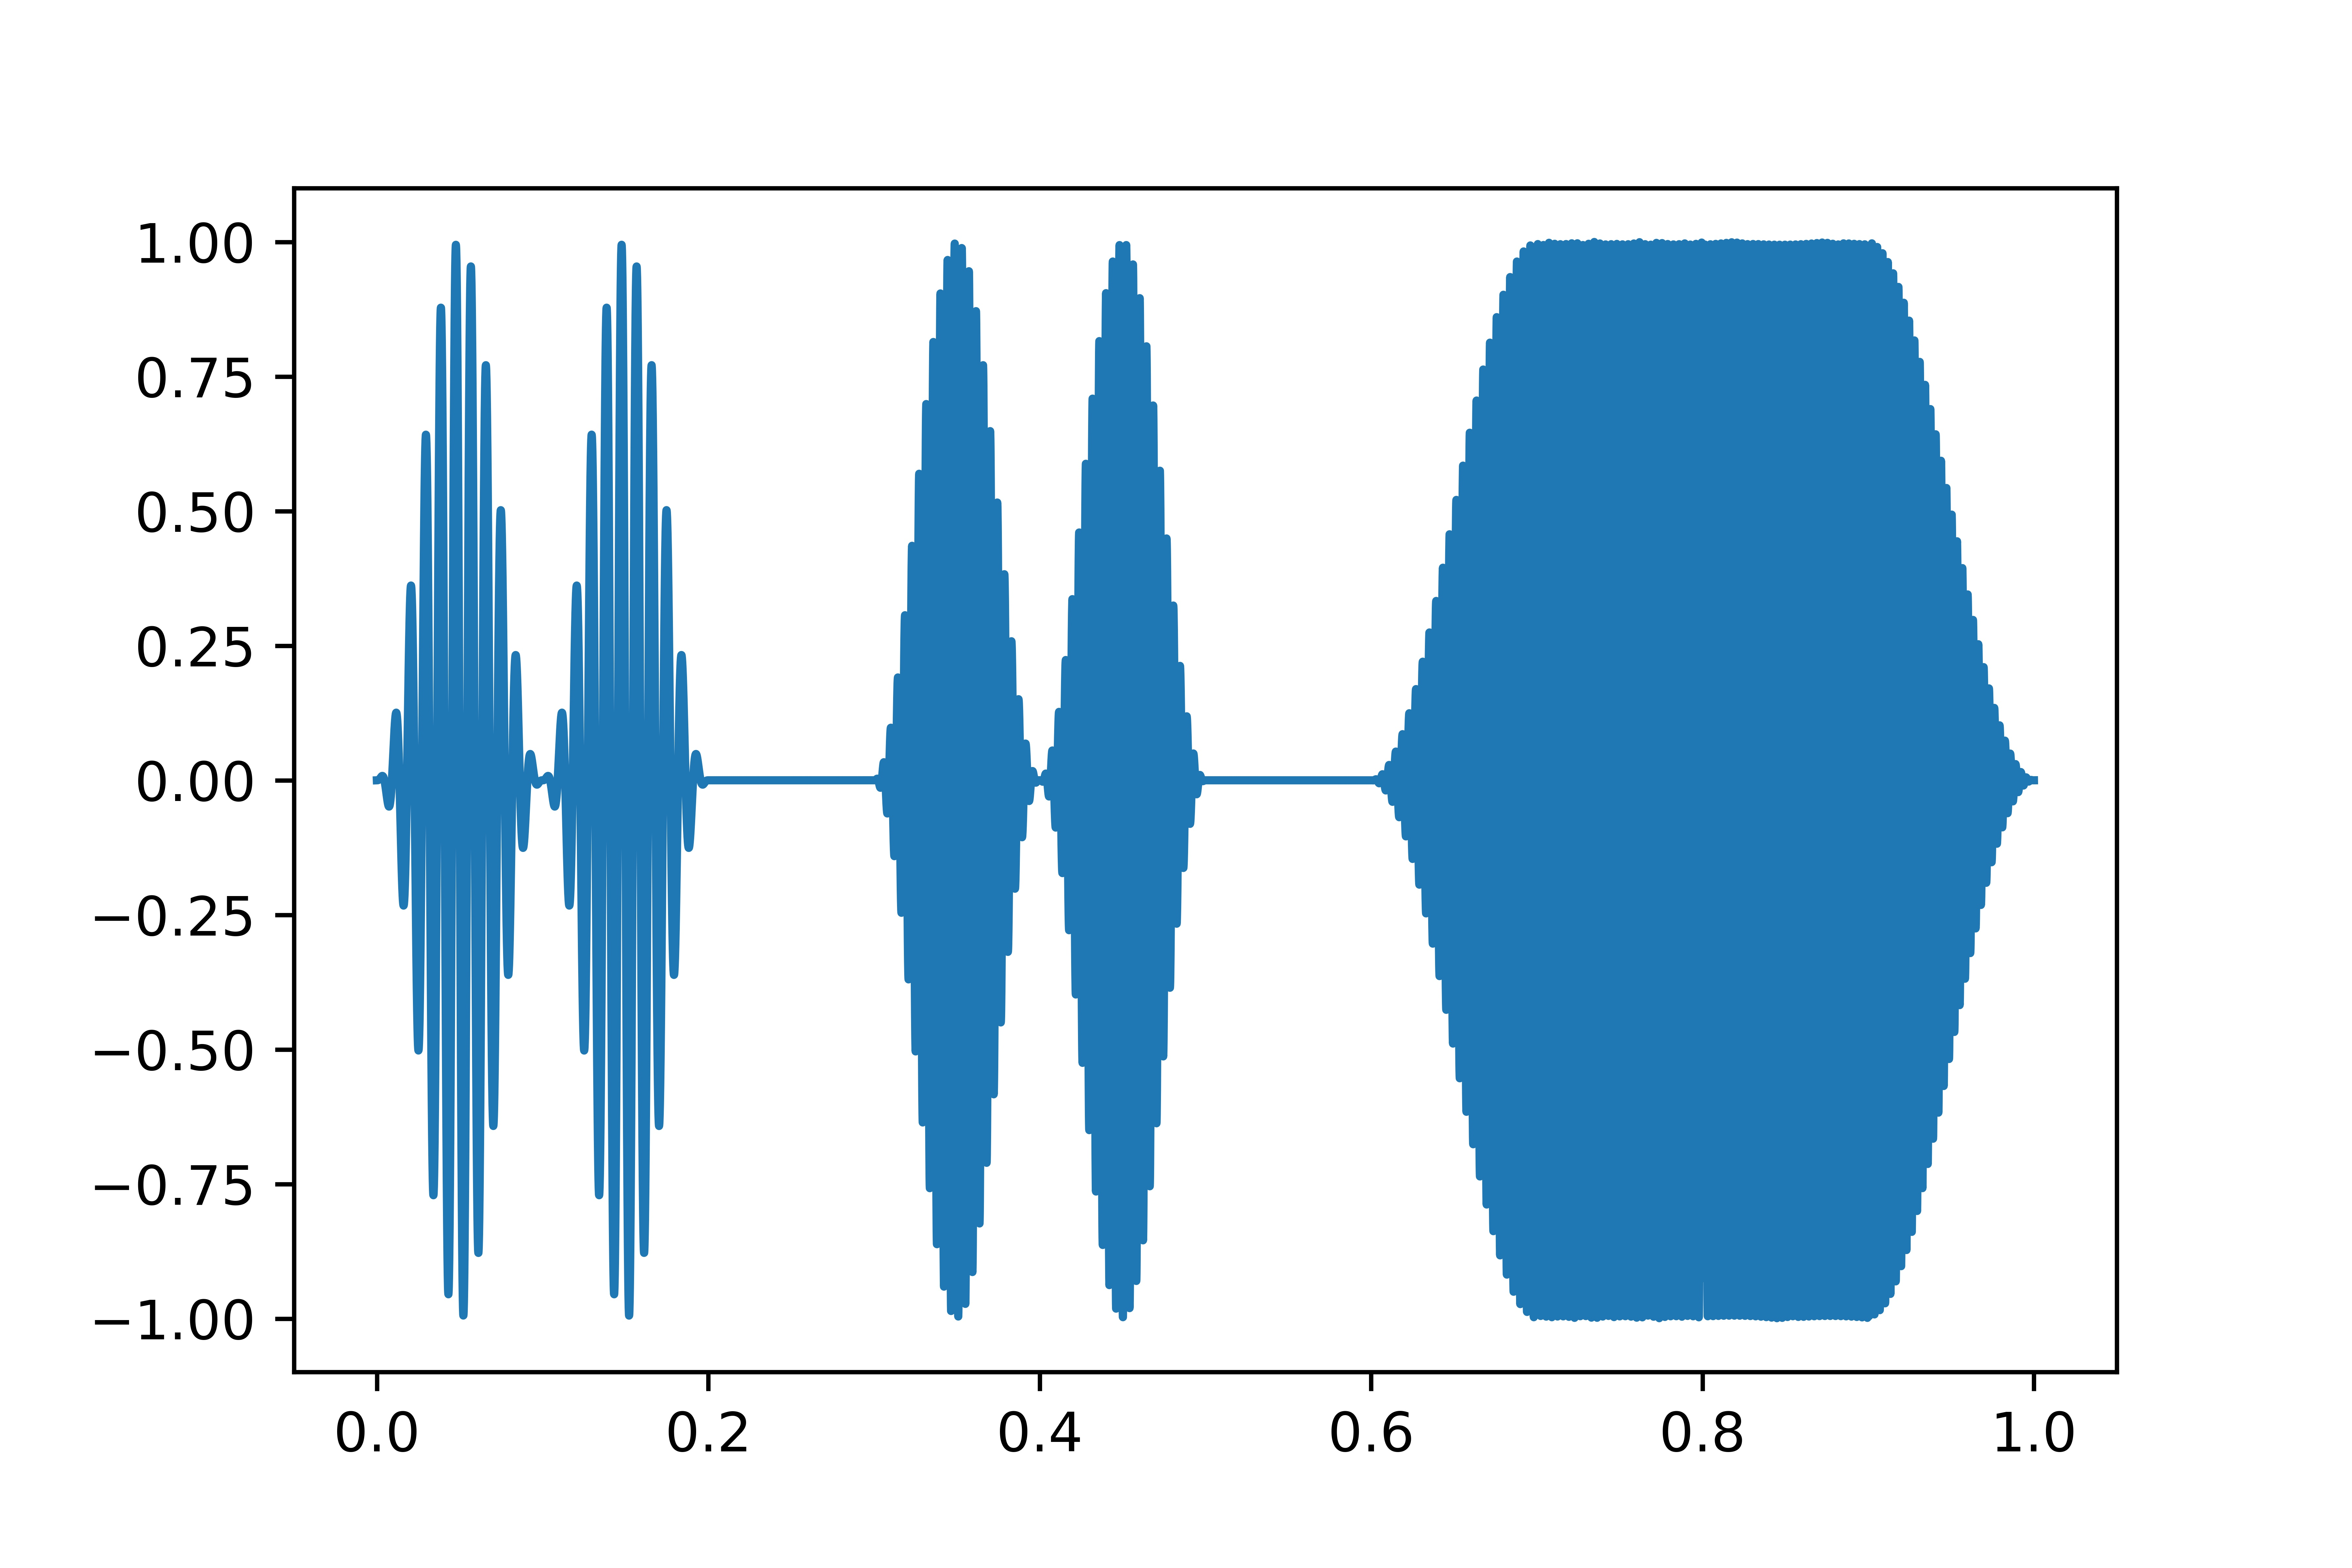
\includegraphics[width=\linewidth]{papers/autotune/sections/frames/images/testsig.jpg}
	\captionof{figure}{Testsignal}\label{fig:frame-testsig}
	\begin{tabularx}{\columnwidth}{XX}
		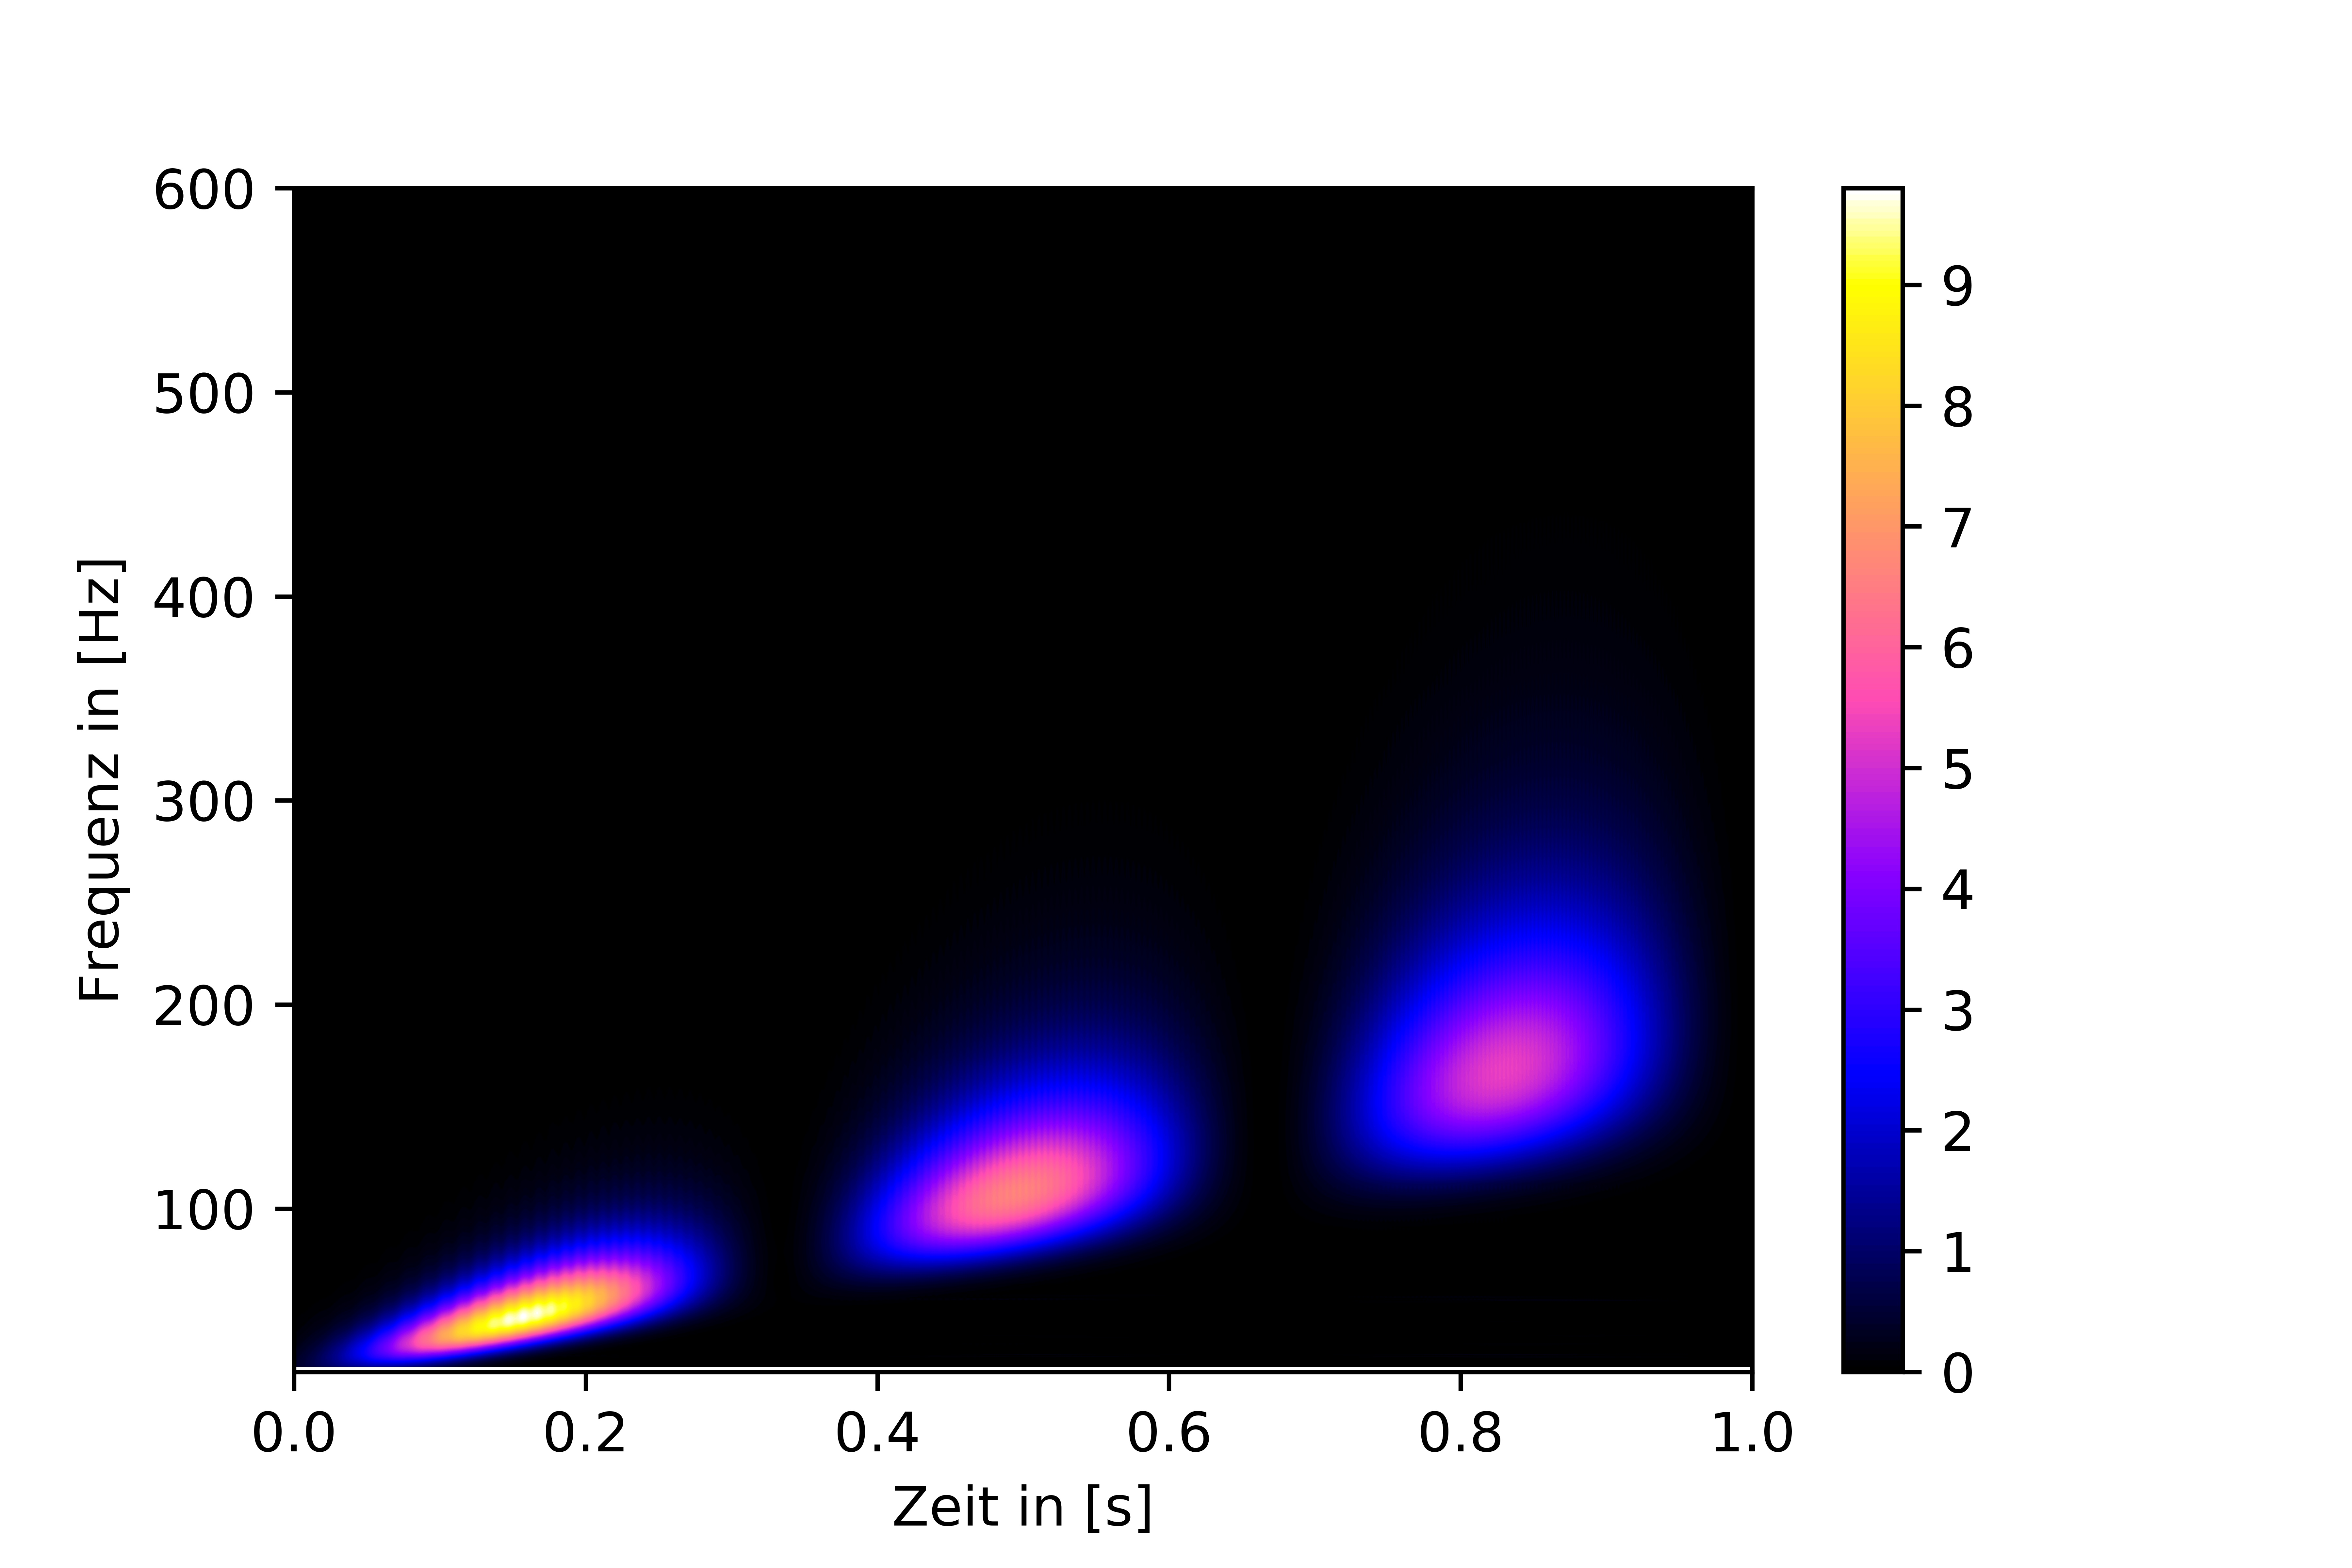
\includegraphics[width=\linewidth]{papers/autotune/sections/frames/images/sincosmcwt.jpg}
		\captionof{figure}{Cwt Analyse mit komplexem Gauss Wavelet des Testsignal}\label{fig:stft256}
		&   \includegraphics[width=\linewidth]{papers/autotune/sections/frames/images/12dwt.jpg}   
		\captionof{figure}{Dauberchi 8 Frame Analyse des Testsignal}\label{fig:cwtsweep}         
	\end{tabularx}
	\caption{Vergleich der Absolutwerte von der cwt und der Frame Analyse mit 12 Basen}
	\label{fig:Frame-Analyse}
\end{figure}%

